\documentclass[12pt,letterpaper, onecolumn]{exam}
\usepackage{amsmath}
\usepackage{amssymb}
\usepackage{graphicx}
\usepackage{setspace}
\usepackage{nicefrac}
\usepackage{hyperref}
\setcounter{MaxMatrixCols}{20}
\usepackage[lmargin=71pt, tmargin=1.2in]{geometry}  %For centering solution box
\lhead{Principles of Navigation}
\rhead{Noah Miller}
\thispagestyle{empty}   %For removing header/footer from page 1

\begin{document}

\begingroup
\centering
\LARGE Principles of Navigation\\
\LARGE Homework 1 \\[0.5em]
\large \today\\[0.5em]
\large Noah Miller\par
\large 903949330\par
\large MECH 6970\par
\endgroup
\pointsdroppedatright   %Self-explanatory
\printanswers
\renewcommand{\solution}{\noindent\textbf{Ans:}\enspace}   %Replace "Ans:" with starting keyword in solution box



\begin{questions}
    \question{Given that 1 minute of latitude is approximately equal to 1 nautical mile\\ (1852 meters), determine the following:}
    \begin{parts}
        \part{%
            How many significant digits after the decimal must be included for a latitude represented in decimal degree to describe a position that is accurate to 1 cm?}\\
        \solution{According to \url{http://wiki.gis.com/wiki/index.php/Decimal_degrees},\\ 7 significant digits are required to have an accuracy of 1.11 centimeters.

        We can do some unit conversion math to confirm this answer. Because we are focusing on displaying the answer in the decimal-degree format, we need to convert our $\frac{1\;[\min-lat]}{1852\; [m]}$ to degrees.
        \begin{equation}
            \begin{split}
                \left(\frac{1\;[\min-lat]}{1852\; [m]}\right)\left(\frac{1\;[deg-lat]}{60\; [min-lat]}\right) & = \left(\frac{0.167\;[deg-lat]}{1852\; [m]}\right)\\
            \end{split}
        \end{equation}
        Since we are trying to find precision to 1 [cm], we then need to convert our $1852$ meters to centimeters.
        \begin{equation}
            \begin{split}
                \left(\frac{0.167\;[deg-lat]}{1852\; [m]}\right)\left(\frac{1\;[m]}{100\; [cm]}\right) & = \left(\frac{9.0173\times10^{-7}\;[deg-lat]}{1\; [cm]}\right)
            \end{split}
        \end{equation}
        According to this conversion, at least 8 significant digits are needed for the latitude to be precise enough to 1 centimeter, although at 7 significant digits would be precise enough to about 1.11 centimeters.
        }

        \part{How many significant digits are required after the decimal in the arc-seconds field if represented in degrees, arc-minutes, and arc-seconds to describe the same accuracy (1 cm)?}

        \solution{
            Because we know at least 8 significant digits are necessary for under 1 centimeter accuracy for the degree-decimal format and $1 \:\text{[deg]} = 60\: \text{[arc-minutes]}$, we can say that 7 significant digits of precision are necessary for an arc-minutes format. Furthermore, because 3600 arc-seconds occupy 1 degree of latitude, we can say the 5 significant digits of precision are necessary when in the arc-seconds format.
        }
    \end{parts}
    Note: $1 \:\text{[deg]} = 60\: \text{[arc-minutes]}$ and $1\: \text{[arc-minute]} = 60\: \text{[arc-seconds]}$
    \clearpage
    \question{Find an outdoor location where you can identify multiple distinctive objects/features in your surroundings. Use a compass, map, and the line of bearing to an object in the field technique discussed in class to triangulate you position in geodectic coordinates (lat/long). You can download topographic maps using this link (\url{https://ngmdb.usgs.gov/topoview/viewer/#4/39.98/-100.06}) You can use the compass on your phone or I have several analog compasses that can be borrowed.}
    \begin{parts}
        \part{Determine your position using two, three, and four features.}

        \solution{
            Standing on the top of the graduate buisness building, I was able to make out Davis Hall, Samford Hall, Jordan-Hare Stadium, and the basketball arena. From these lines of bearing I was able to determine my to position to be roughly $32.606^o$ N and $84.490^o$ W.
            \begin{figure}[!h]
                \centering
                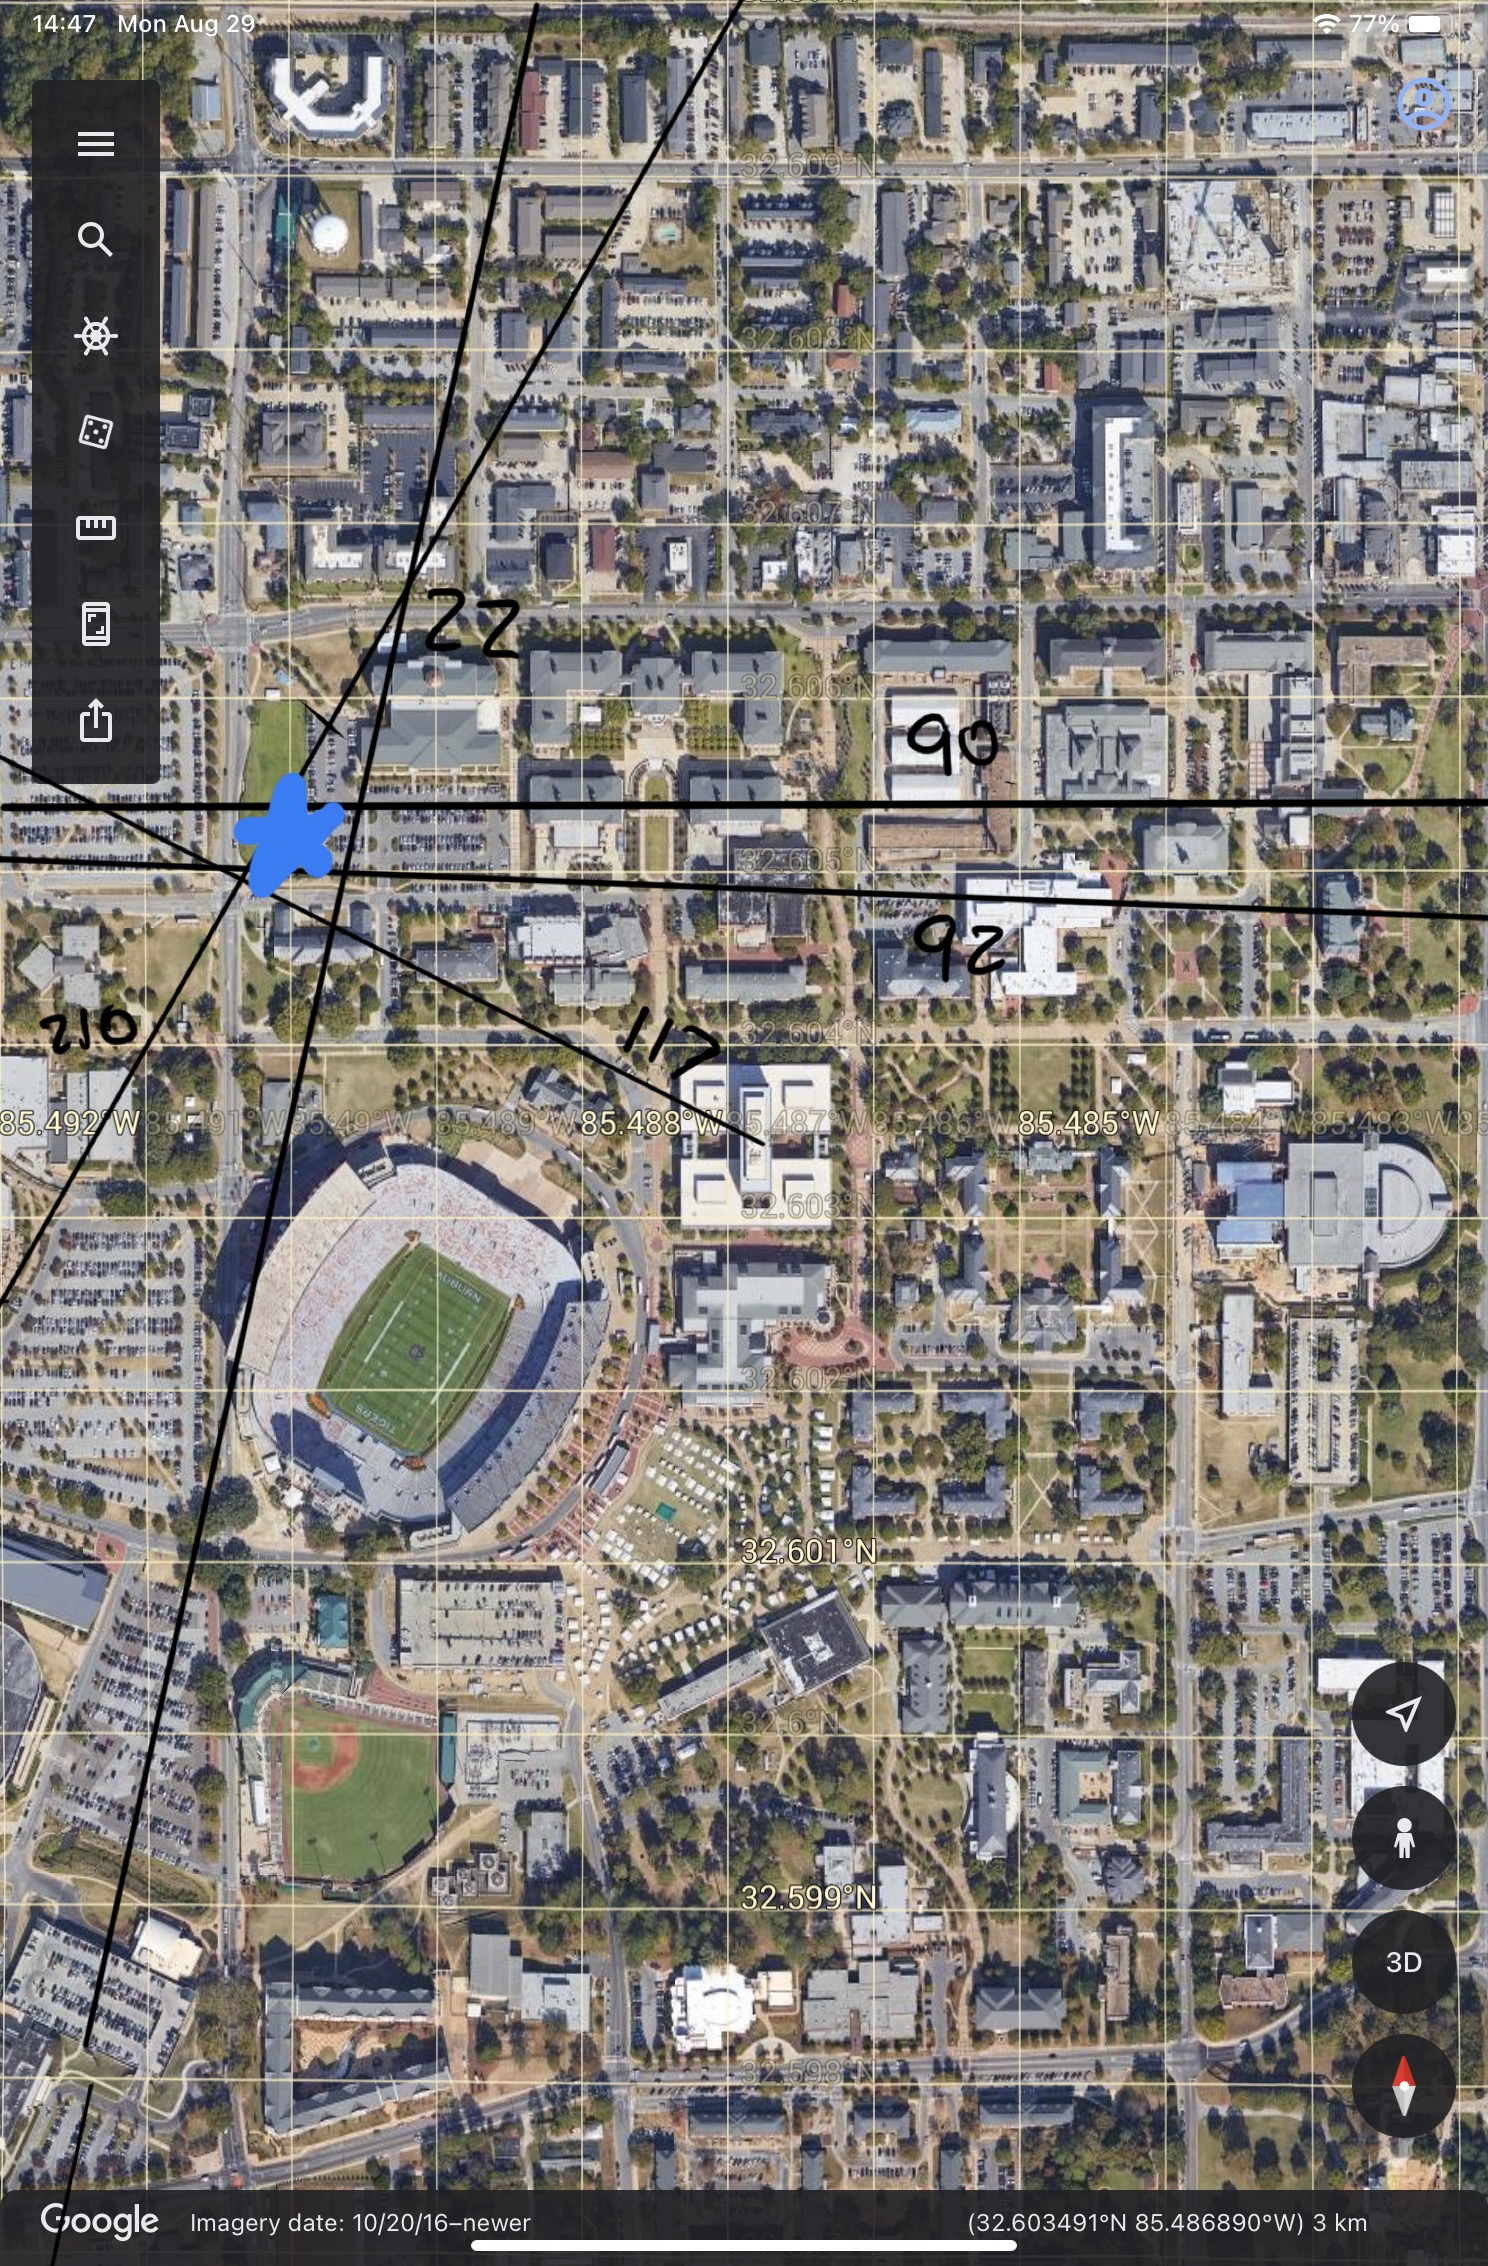
\includegraphics[width=.5\linewidth]{IMG_0025 2022-08-30 03_13_02.jpg}
            \end{figure}
        }
        \clearpage
        \part{Compare the accuracy of those solutions to your true location. You may use GPS, Google Maps, or other references to determine your "true" position.}

        \solution{
            Using the compass app on my iPhone, it displayed a true location of $32.605556^o$ N and $85.49^o$ W.
            \begin{figure}[!h]
                \centering
                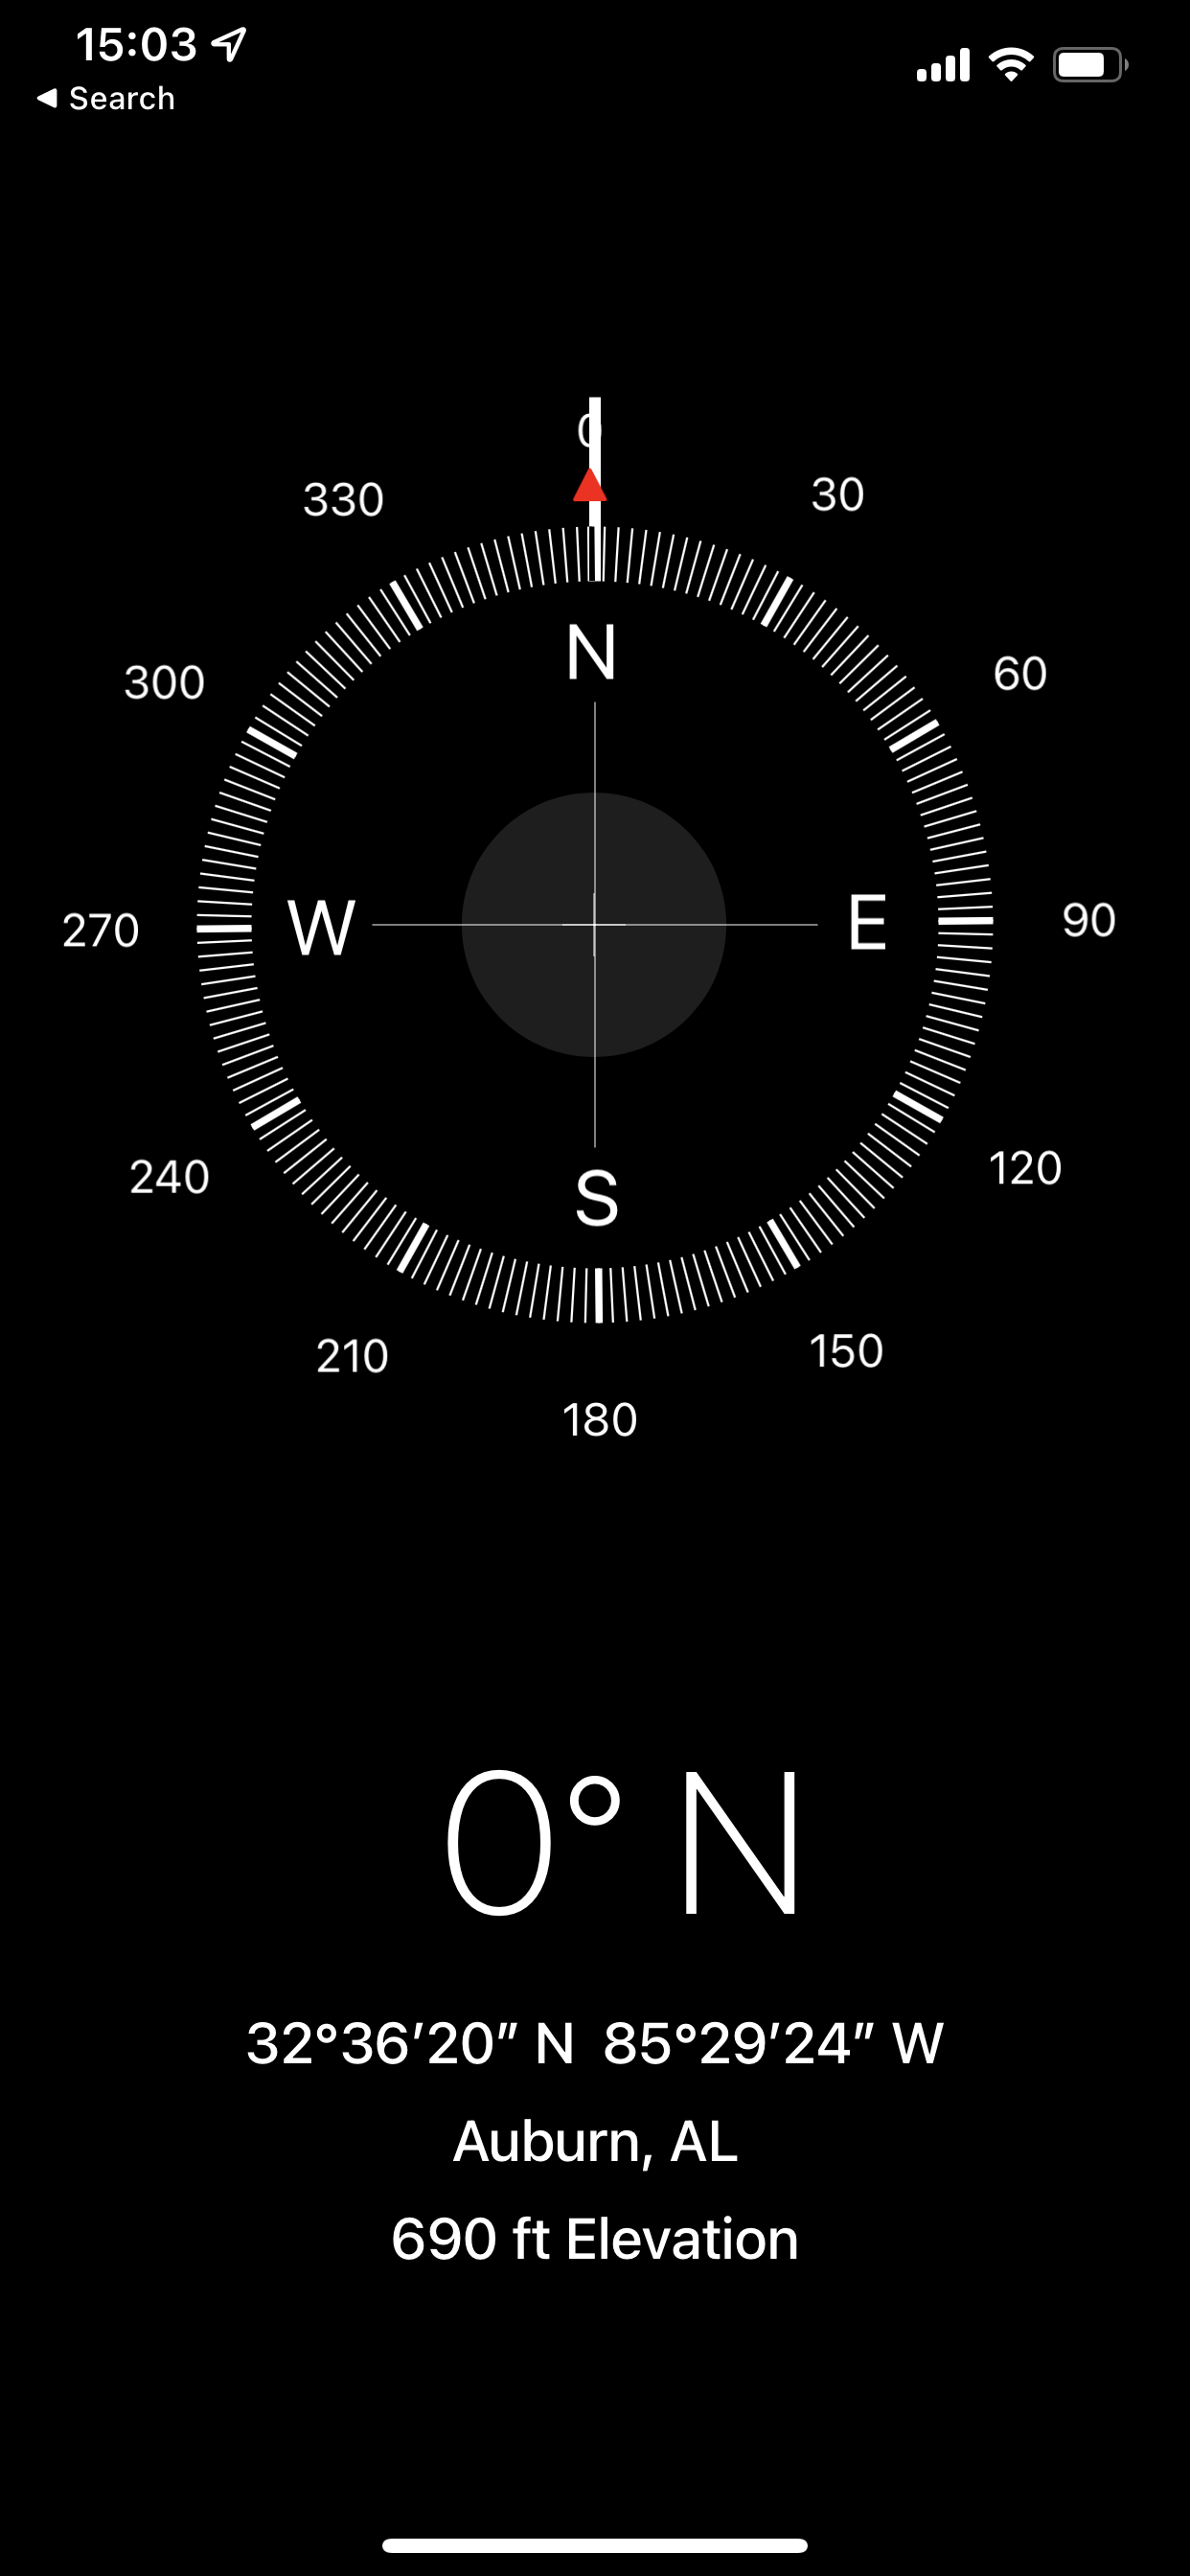
\includegraphics[width=.3\linewidth]{IMG_7250 2022-08-30 03_13_03.PNG}
            \end{figure}
        }
        \clearpage
        \part{To how many significant digits was your estimated position accurate?}

        \solution{Comparing my estimated and true position reveals that my latitude was accurate to 5 significant digits and my longitude to 4 significant figures. I was surprised to see the accuracy of my estimated position. I believe this was due to the Google Earth app having very precise lines of latitude and longitude. This made it easy to make an estimate of my location by taking the average of the two lines of longitude out side of my predicted location.}
    \end{parts}
    \clearpage
    \question{Find and discuss a documented instance of a failure of navigation in a trans-oceanic flight. Be specific as to what went wrong and how this affected mission.}\\
    \solution{
        According to \url{https://www.history.com/}, The first nonstop flight across the Atlantic ocean was a harrowing journey that lasted for 16 hours, not just due to "rudimentary aircraft", but also its archaic navigation system. Originally the two pilots, Alcock and Brown, were set to takeoff in Newfoundland and land near London. However, "fog overwhelmed the pilots, making navigation—conducted by sextant—next to impossible". Because the pilots were unable to accurately attain their position, they played it safe and landed at the first inkling of land they saw - which turned out to be Clifden of West Ireland. Clifden is about 900 kilometers west of London.}
    \clearpage
    \question{Find and discuss a documented instance of a failure of guidance in a trans-oceanic flight. Be specific as to what went wrong and how this affected the mission.}

    \solution{ This example could be up for debate, but the Malaysia Airlines Flight 17\\
    (\url{https://en.wikipedia.org/wiki/Malaysia_Airlines_Flight_17}) was a guidance failure that resulted in the flight being shot down over Eastern Ukrainian airspace by Russian Separatists. The flight is a Boeing 777-200ER and took off from Amsterdam and was supposed to land in Kuala Lumpur. The original flight plan proposed the airplane to fly around the conflict area and at a higher flight level, such to avoid the conflict area better. Upon nearing the conflict area, the pilots asked to stay at their current altitude of 33,000 [ft] (330 FL) and move to 20 [nm] north of their original track - ATC approved. The guidance system failed and the last contact with the airplane was found at FL 330 but almost 3.5 miles north of its proposed track, into the conflict area, where it was shot down. Autopilot and controls systems are advanced enough on these airplanes for it not to be a control problem, regardless of weather or wind conditions. My guess is that guidance system, around being updated to stay at the same flight level, reprogrammed itself to find the shortest route to the Kuala Lumpur airport.

    }
    \clearpage
    \question{Assume that you have 1000 noisy biased measurements of the acceleration (scalar) of a \textit{\textbf{stationary}} body over 100 seconds ($dt = 0.1$) as shown in the equation below.
        \[\tilde{\ddot{x}} = \ddot{x} + b + \eta \]
        \[b = 3 \]
        \[\eta \sim N(0,1) \]
        Numerically integrate the noisy biased measurements of acceleration to calculate velocity and position (assume zero initial conditions). Repeat this process 100 times such that you have 100 random velocity and position values from each time step. calculate the variance of the velocity and position at each time step and plot them versus time.

        Note: $N(0,1)$ indicates a normal distributed random variable with zero-mean and a variance of 1. The MATLAB command $>>randn$ generates normally distributed samples with a variance of 1.}

    \solution{%
        Because velocity and position have a dependency on the acceleration measurement, the noise gets inheiritly integrated at each time step, leading to a huge amount of variance at the end of the measurement period.
        \begin{figure}[!h]
            \label{fig:3}
            \centering
            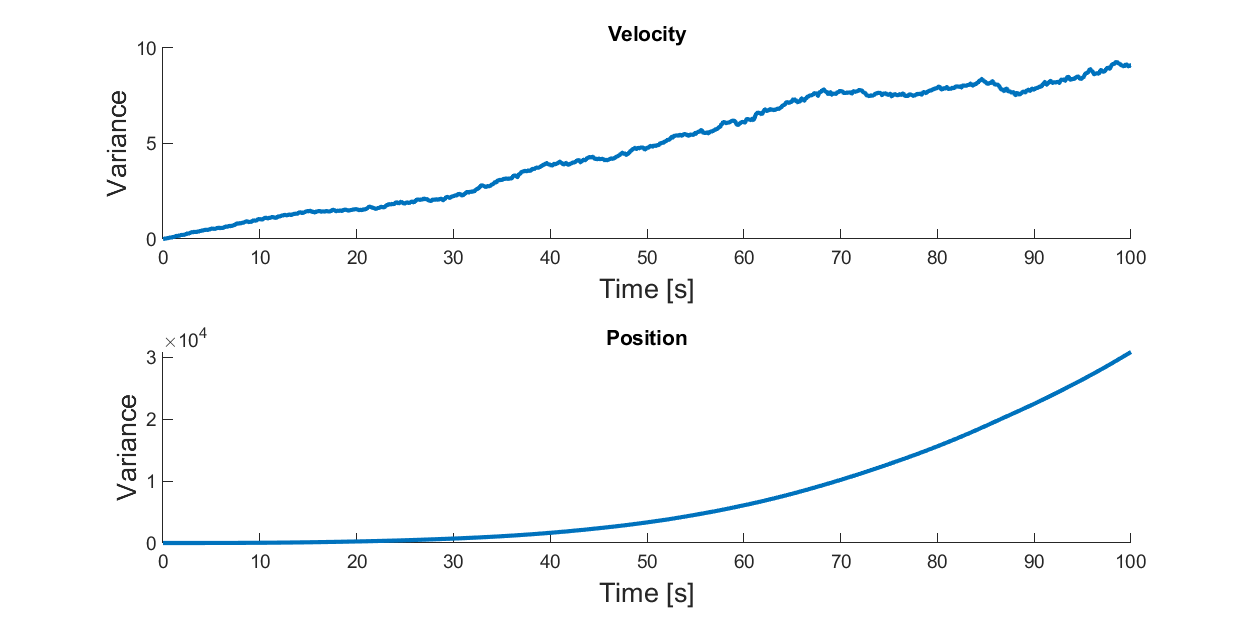
\includegraphics[width=\linewidth]{Q5.png}
        \end{figure}
    }
    \clearpage
    \question{Given the simulate acceleration measurements for problem 5, do the followiing:}
    \begin{parts}
        \part{How would you estimate the bias?}

        \solution{%
            Because the body is known to be stationary, we can take the mean of the acceleration measurements. If the body was moving, computing a least squares solution could be another option.
        }

        \part{Compute the 100 estimates of the bias using each set of 1000 measurements.}

        \solution{%
            From the figure below, we can see the monte-carlo simulation reveal a bias of around 3, which is the bias provided in the problem statement.
            \begin{figure}[!h]
                \centering
                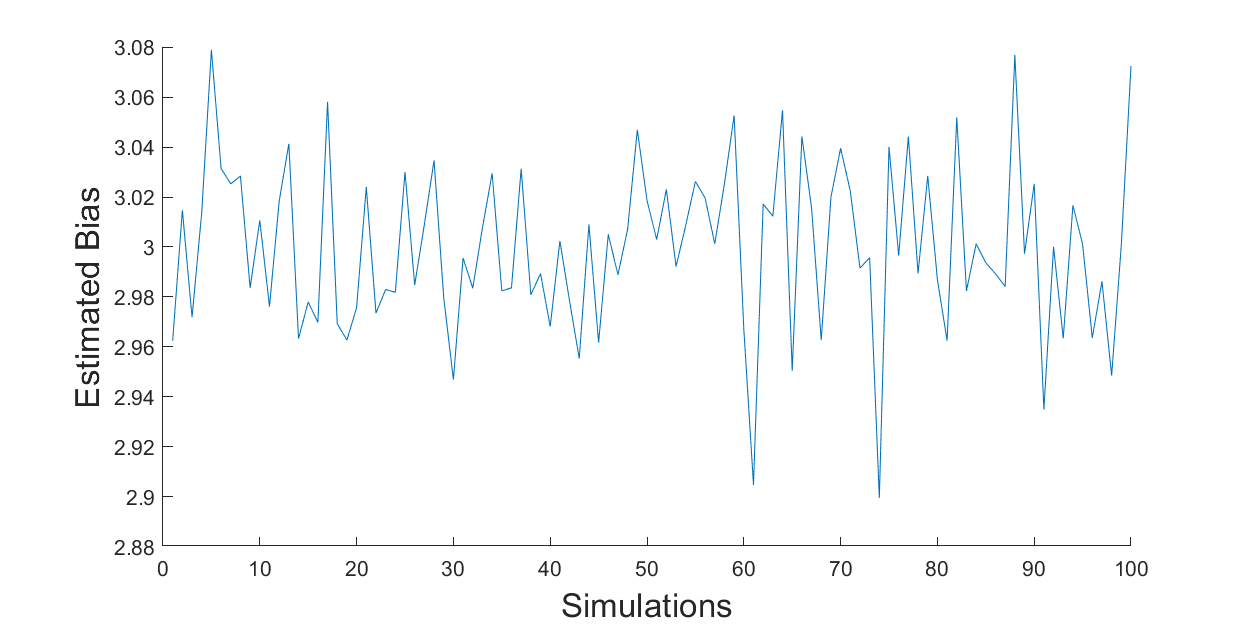
\includegraphics[width=\linewidth]{Q6b.png}
            \end{figure}

        }

        \part{What is the mean and variances of the bias estimates?}

        \solution{%
            Taking the expectation of our monte-carlo bias estimate gives us an average bias estimate of $3.003$ which is more near our set bias value. The variance of the monte-carlo simuations was $9.53\times10^{-4}$. We could lower the variance closer to 0 if we run more simulations.
        }
    \end{parts}
    \clearpage
    \question{You set out from town \textbf{A} and head east to town \textbf{B} $120$ kilometers away. Your vehicle has an odometer that is not particular accurate (it could be off by 1-2 kilometers after 50 kilometers of driving). You carry a decent watch, which is great at keeping time over short intervals, but it has been months since you last reset it. In other words, you can measure time intervals accurately, but do not know exactly what time it is. A short into your journey, the car breaks down.}
    \begin{parts}
        \part{According to your odometer, you have traveled 56 kilometers. Estimate your position.}

        \solution{%
            Becuase the odometer has a variance of $\pm 2$ [km], our position could be $54$ to $58$ [km] east of town \textbf{A}.
        }
        \part{As you push your car to the shoulder of the road, a red bus zooms by, traveling from town \textbf{A} to town \textbf{B}. You glance at your watch and notice that it is exactly 21 minute past the hour. You know that the red buses are prompt, and they leave town \textbf{A} every hour on the hour traveling at exactly 3 kilometers per minute. Can you estimate your position without using the odometer information?}

        \solution{%
            Assuming that it is \textit{actually} 21 minutes past the hour, you could estimate your position to be $63$ [km] east of town \textbf{A}.
        }

        \part{Estimate your position and clock bias based on all the information so far.

            (Hint: Write two equations that relate your position and clock bias to the available information. These equations are sometimes referred to as a navigation equations.)}

        \solution{%
            Using our estimated postion from our car's odometer and the speed of the bus along with our watch, we can write out kinematic equations to estimate our clock bias.
            \begin{equation}
                \begin{split}
                    s & = s_{odom}\\
                    s & = v_B(t_W + b_W)\\
                    s_{odom} & = v_Bt_W + v_B b_W\\
                    56 & = 3 \left[\frac{km}{min}\right] \cdot 21 \left[min \right] + 3 \left[\frac{km}{min}\right] b_W \left[min \right]\\
                    b_W & = -2\frac{1}{3} \left[min\right]\\
                    & = -2 \left[min\right] 20 \left[s\right]\\
                \end{split}
            \end{equation}
            Based on the above work, the clock bias on the watch could at most be 3 minutes fast and at least 1 minute 40 seconds fast. Assuming the odometer to be accurate tells us that our watch is 2 minutes and 20 seconds fast.
            \begin{equation}
                \begin{split}
                    s & = v_B(t_W + b_W)\\
                    s & = 3 \left[\frac{km}{min}\right](21 \left[min \right] + -2\frac{1}{3} \left[min\right])\\
                    s & = 56 \left[km\right] \pm 2 \left[km\right]\\
                \end{split}
            \end{equation}
        }
        \part{At 25 minutes past the hour according to your watch. You observe a blue bus zoom past at 2.5 kilometers per minute, going from town \textbf{B} to town \textbf{A}. Blue buses leave town \textbf{B} every hour on the hour promptly and drive to town \textbf{A} at a constant speed. Estimate your position and clock bias based on all the information so far. (Hint: Recall that your watch can measure $dt$ accurately.)}

        \solution{%
            We can use all three measurements to estimate our clock bias and position in a similiar fashion to part (c).
            \begin{equation}\label{eq:5}
                \begin{split}
                    s_{blue}    & = v_{blue}(t_{blue}) + 120\\
                    & = -2.5 \left[\frac{km}{min}\right]\cdot25\;[min]+ 120\;[km]\\
                    & = 57.5\; [km]\\
                \end{split}
            \end{equation}
            In equation~\ref*{eq:5} we add in $120\;$[km] to represent the distance between the towns and the velocity for the blue bus is negative to represent vehicles coming from town \textbf{B}.
        }

        \part{How would your solution be affected if your watch were exactly five minutes fast and all the clocks in town \textbf{A} and town \textbf{B} were running five minutes fast?}
        \part{Now suppose that your odometer never worked and the only vehicles you see are identical yellow cabs of carrier L1. These cabs leave town \textbf{A} every minute on the minute and travel exactly 1 kilometers per minute to town \textbf{B}. Can you estimate your position and clock error? Would it help if there were identical green cars of carrier L2 leaving town \textbf{B} every minute on the minute and traveling at 1 kilometers per minute to town \textbf{A}?

            Explain briefly.}
    \end{parts}
\end{questions}
\end{document}